\documentclass[10pt]{article}
\usepackage{multicol, caption}
\usepackage[margin=1in]{geometry}
\usepackage{graphicx}
\newenvironment{Figure}
  {\par\medskip\noindent\minipage{\linewidth}}
  {\endminipage\par\medskip}
\graphicspath{ {images/} }
\title{\textbf{Real-time Mesh Deformation using Volumetric Graph Laplacian}}
\author{Elias Eberhardsson}
\date{}
\begin{document}
\maketitle

\textit{
This paper describes the implementation and testing of a mesh deformation method using volumetric graph laplacian for use in real-time. First a graph of nodes in a crystal structure inside the 3D mesh is constructed. The nodes are connected together and linked with the mesh. These nodes and their connections are used to preserve volumetric detail when deforming vertices contained in the mesh. The laplacian on vertices based on this graph is how volumetric details are preserved, coupled with the laplacian on the mesh, which preserves outer details. And such the deformed locations are calculated. This method should ideally be used together with quadratic minimization, but due to the time constraint this was left out in favour of a simple interpolation of new vertex position and the two laplacian values.
}
\begin{multicols}{2}
\section{Introduction}
Mesh deformation has been interesting to computer scientists for as long as we have been able to draw vertices on the screen. Much research has been done and many many methods have been created and put forth through scientific publications. 

There are many applications for mesh deformation: animation, modelling and simulations are some of the more prominent ones.

The method showcased in this paper aims to in real-time deform a mesh while balancing volumetric and surface details and such prevent self-intersection and unnatural looking bends and twists. 
The method builds on the Volumetric Graph Laplacian (VGL), used in [Zhou et al. 2005], which owes itself to differential domain techniques and graph theory. This represents detail as points differences from origo to be balanced between.
\section{Related work}

This project is an attempt at implementing the method described in the paper Large Mesh Deformation Using the Volumetric Graph Laplacian [Zhou et al. 2005] which was an attempt at much better preserve detail and volume when doing deformations such as bending and twisting parts of a mesh. This method used quadratic minimization on energy functions to as closely as possible simulate a real deformation.

Supposed to be used but cut due to time constraints are WIRE deformation [Singh and Fiume 1998] where a method of connecting vertices in a mesh on a curve and deforming with some constraints to how the curve may bend. This combined with volumetric graph laplacian is what is described in [Zhou et al. 2005].

As mentioned in the introduction this is also closely related to differential domain techniques [Yu et al. 2004] and spectral graph theory [Chung 1997].

\section{Deformation on Volumetric Graphs}

Given a mesh \textit{M = (V, K, N)}, where \textit{ \[ V = \{ p_i \in R^3|1\leq i \leq n \} \] } are the vertex positions as points in 3D-space and \textit{K} is the connective data to each of the adjacent volumetric nodes in the 3-dimensional array that is used to store them: \textit{ \[ K = \{ I_i \in R^3|1\leq i \leq m \} \] } And \textit{N} is similarily the conncetive data to adjacent vertices in the mesh: \textit{ \[ N = \{ N_i \in R|1\leq i \leq k \} \] } Using this as a starting point we can lay out the details of the deformation method.
\subsection{Volumetric graph}
\begin{Figure}
	\centering
	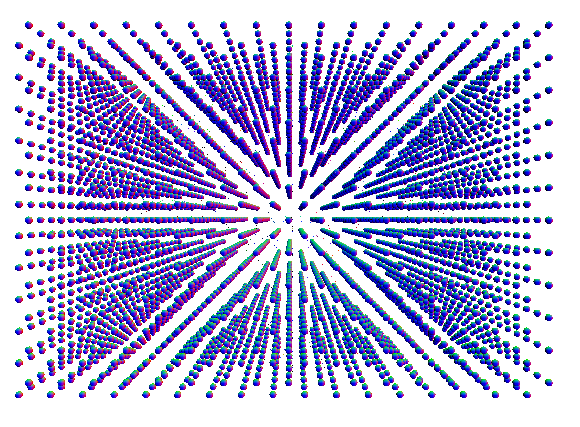
\includegraphics[width=\linewidth]{graph1.png}
	\captionof{figure}{Graph structure.}
\end{Figure}
\begin{Figure}
	\centering
	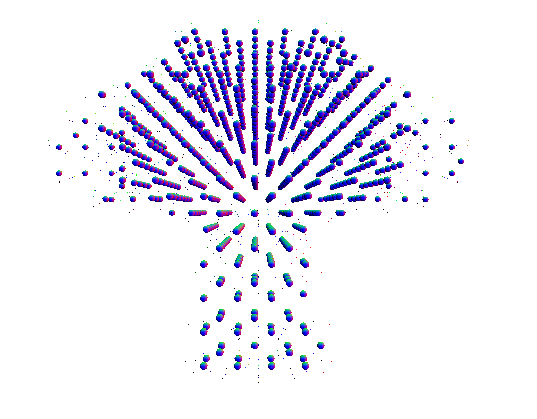
\includegraphics[width=\linewidth]{graph2.png}
	\captionof{figure}{Final volume graph.}
\end{Figure}
To construct the graph that is used to represent volume in the deformation we build two 3-dimensional fields of nodes. The distance, \textit{d}, between each node is set to the average edge-distance in the mesh. The fields are offset by half of \textit{d} in each direction to create a structually sound, crystal-like, volume, see figure 2.
 
When this is done all nodes which are not contained within the mesh are discarded. Finally each node in the resulting graph are connected to each of its neighbors and any mesh-vertices within \textit{d\textbackslash2} is connected and that vertex is also given information on which connections that have been made, see figure 3.

The method used to determine whether a node is contained within the mesh is to calculate triangle-ray intersections from the node in an arbitrary direction. Given an even number of intersections the node is outside of the mesh, and given an uneven number, the node is contained within the mesh.

\subsection{Laplacian of graph}
The laplacian of a graph is the same as the laplacian operator on manifolds [Chung 1997] and computes the difference of a point \textit{p} and all of its adjacencies. Given a weight \textit{w} for each neighbor that satisfies \[ \sum_{j\in N_i \cup K_i} w_{ij} = 1\] we linearly compute the difference of the graph adjacencies: \[ \bigtriangledown_G(p_i) = p_i - \sum_{j\in K_i}w_{ij}p_j \] Similarly we do this for mesh adjacencies: \[ \bigtriangledown_M(p_i) = p_i - \sum_{j\in N_i}w_{ij}p_j \] Here $\bigtriangledown$ is the laplacian operator and \textit{G} and \textit{M} is the volumetric graph and the 3D mesh respectivly.

This gives us two terms, one which encodes volumetric detail and one that contains surface detail.
\subsection{Deformation}
Given a point \textit{q\textsubscript{i}} that is the target deformation point for \textit{p\textsubscript{i}} we need to find the point \textit{p`\textsubscript{i}} that balances volume and detail but still deforms \textit{p\textsubscript{i}} satisfactorily. 

We have the three terms a, b, and c: 
\[ a = \bigtriangledown_G(h_{i}) - \bigtriangledown_G(p_i)\]
\[ b = h_i - q_i\]
\[ c = \bigtriangledown_M(h_{i}) - \bigtriangledown_M(p_i)\]
where \[ h_i = p_i + \gamma*(p_i - q_i)\]
$\gamma \in \{ 0..1 \}$ gives $h_i$ an approximate value of a deformed location. $\gamma$ is set to 0.6 in our implementation.

The final deformed location $p`_i$ is calculated:
\[ p`_i = a*(1 - \alpha - \beta) + b*\alpha + c*\beta \]
$\beta$ balances between surface and volume details. $\beta = n/N$ works well where n is the number of vertices on the mesh and N is the count of the volumetric nodes contained in the graph. 

Experimenting with $\alpha$ is needed to achive good results based on the mesh that is to be deformed, but 0.4 seems like a good number, as used in [Zhout et al. 2005].

\subsection{Propagation}
When a new position has been calculated we use it to get the relative translation needed to be done. $T = p`_i - p_i$. The translation \textit{T} is propagated throughout the mesh using a simple propagation scheme. So that each of $p_i$'s neighbor $n$ is translated $T*(1/||p_n - p_i||)$.

\section{Results}

The results were subpar if you were to compare this to any proper implementation using energy functions and quadratic minimization. Also a better way to propagate would have been great to get good looking reults. 

\begin{Figure}
	\centering
	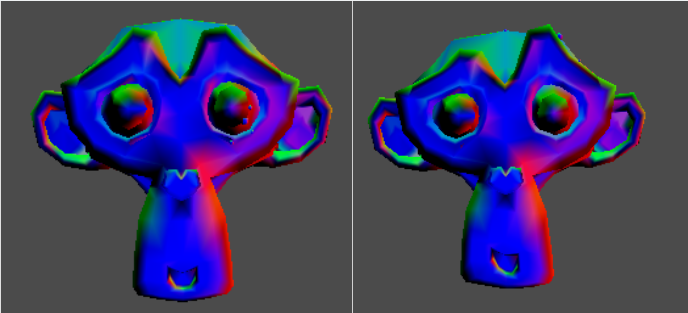
\includegraphics[width=\linewidth]{mondef.png}
	\captionof{figure}{Face deformation.}
\end{Figure}

Small deformations work fine, moving parts of a face as an example looks fine, as shown in figure 4. But trying to bend bigger shapes do not come out good without much tweaking to the balancing and changes to the weight used in propagation, shown in figure 5 and 6.

\begin{Figure}
	\centering
	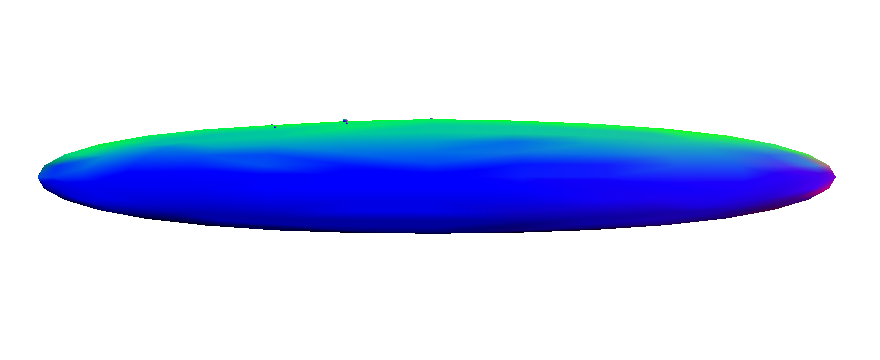
\includegraphics[width=\linewidth]{korv1.png}
	\captionof{figure}{Pre deformed.}
\end{Figure}
\begin{Figure}
	\centering
	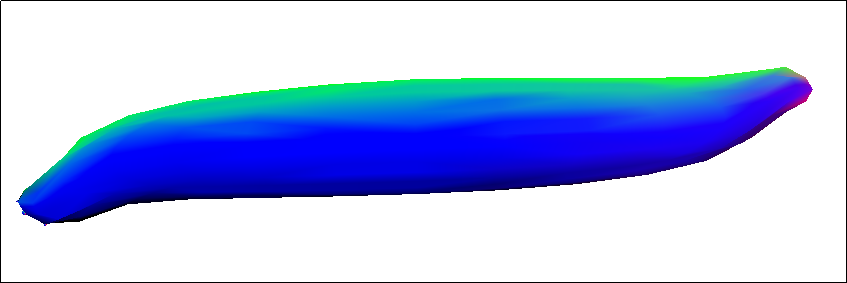
\includegraphics[width=\linewidth]{korv2.png}
	\captionof{figure}{Post deformed.}
\end{Figure}

\section{Conclusion and Reflections}

Our implementation of these deformation algorithms are subpar at best. We underestimated the work and planning needed to properly implement and use VGL [Zhou et al. 2005], completely missing the need for WIRE deformation to do large deformations the first ten times I read the paper.

We had intended to use quadratic minimization on energy functions, as laid out in [Zhou et al. 2005], but we did not understand the bounds used nor had we enough time to implement or get used to any library needed for such computation. And as such our simple interpolation does prove decent at preserving volume and detail in small deformation and does prevent self-intersection. But it fails at any large deformation, or any greater deformations tried, which results in odd looking results.

Instead of simply a translation to be propagated, it should be a transformation-matrix, otherwise proper turning and twisting would have a hard time looking proper.

If I got to do this all over again, I would plan in much greater detail all parts of the implementation, choice of datastructures used and all things that actually needed to be understood.

\begin{thebibliography}{7}
\bibitem{zhou} 
Kun Zhou, Jin Huang, John Snyder, Xinguo Liu, Hunun Bao, Baining Guo and Heung-Yeung Shun. 2005.
\textit{Large Mesh Deformation Using the Volumetric Graph Laplacian}. 
ACM Trans. Graphics (Proc. ACM SIGGRAPH), vol. 24, no. 3, pp. 496-503.
 
\bibitem{moller} 
Tomas M{\"o}ller. 1997.
\textit{A Fast Triangle-Triangle Intersection Test}.
Journal of Graphics Tools, 2(2):25-30.
 
\bibitem{moller2}
Tomas M{\"o}ller and Ben Trumbore. 1997.
\textit{Fast, Minimum Storage Ray/Triangle Intersection}.
Journal of Graphics Tools, 2(1):21-28.

\bibitem{chung} 
Chung F.R.K. 1997.
\textit{Spectral Graph Theory}.
CBMS 92, AMS.

\bibitem{gingh} 
Karan Singh and Eugene Fiume. 1998.
\textit{Wires: A Gerometric Deformation Technique}.
SIGGRAPH 98 Conference Proceedings, pages 405-414.
\end{thebibliography}



\end{multicols}
\end{document}
